\section{Brain Design} \label{sec:brain}
What follows is a series of descriptions of each of our brain models and what
features they added to the agent's functionality. In general, we wanted to 
start with a brain dead agent, then add to it movement, consumption, 
perception, and eventually judgement. Our figures in this section are used to 
illustrate the elements we have adjusted for each model. The full 
architecture of each model can be seen in appendix~\ref{ap:arch}.

\subsection{Brain 0}
We started from the most simplistic of models: an agent who sits in place until
it dies. It shuns all of its inputs, and uses none of its actuators.

\subsection{Brain 1}

Our second brain (Fig. \ref{fig:brain1}) constantly activates the agent's 
eating actuator (i.e. the agent will try to eat anything with which it comes
in contact). It also moves in a straight line.

\begin{figure}
\begin{center}
  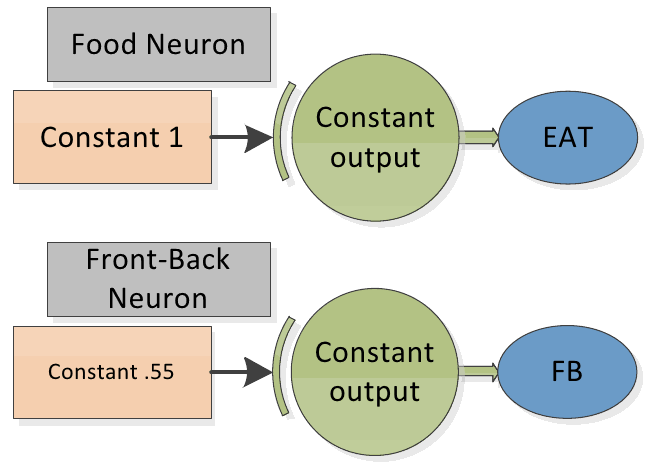
\includegraphics[scale=.3]{img/brain1.png}
  \caption{Active neurons in Brain 1}
  \label{fig:brain1}
\end{center}
\end{figure}

\subsection{Brain 2}

Brain 2 was the first neural network to take advantage of the agent's visual
cortex (Fig. \ref{fig:brain2}). Of the 31 eyelets available to the agent, it 
used only the data it received from its center eyelet (eyelet 15). This
neuron instructs the agent to only use its eat actuator when it percieves
intense brightness. 

We caused this behavior by using a single neuron with a step function. 
The neuron was trained by having the agent try to eat at a variety of 
distances and observing the change in its charge. If the charge does not
change, then the brightness threshold is increased.

\begin{figure}
\begin{center}
  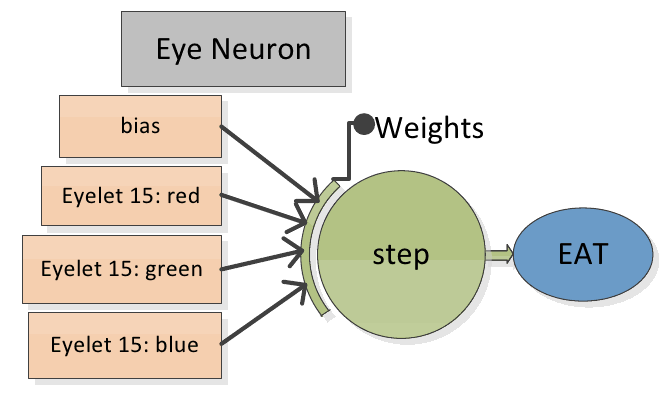
\includegraphics[scale=.3]{img/brain2.png}
  \caption{Brain 2's visual neuron}
  \label{fig:brain2}
\end{center}
\end{figure}

\subsection{Brain 3}

For our fourth brain, we actually made two changes. The first was to the
eye neuron, which we changed from a step function to a sigmoid 
(Fig. \ref{fig:brain3eye}):

\begin{equation} \label{eq:eyesig}
  \varphi(v) = \frac{\tanh(2v)}{10}
\end{equation}

We made this change because we wanted this model to focus on color. Whereas
our old step function classified \emph{all} objects as ``close enough'' vs. 
``not close enough,'' this new version looked could classify the input by 
consuming it, comparing the output to the change in energy. Since this change 
can only be -0.1, 0, or 0.1, we selected a sigmoid function that would return 
a value within that range. Using a continuous function like \eqref{eq:eyesig} 
allows us to compare colors of objects.

\begin{figure}
\begin{center}
  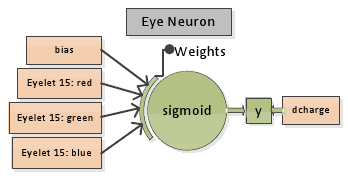
\includegraphics[scale=.7]{img/brain3eye.png}
  \caption{Brain 3's visual neuron}
  \label{fig:brain3eye}
\end{center}
\end{figure}

Our second change was to employ the somatic sensors of the agent
\ref{fig:brain3touch}. If the agent senses contact on any of its edges, it 
will eat. By using these somatic sensors, we keep our agent from slovenly
gnashing its teeth at every time step.

\begin{figure}
\begin{center}
  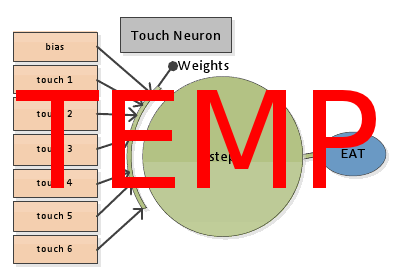
\includegraphics[scale=.65]{img/brain3touch.png}
  \caption{Brain 3's somatic neuron}
  \label{fig:brain3touch}
\end{center}
\end{figure}

\subsection{Brain 4}

Our mission for Brain 4 was to implement the rest of the eyelets into a
winner-take-all network (Fig. \ref{fig:brain4}). Each eyelet input is fed 
into two neurons: one sigmoid to determine color, and another which produced 
the linear summation of each color's intensity. The product of these two 
neurons' outputs is then fed into a 31-element WTA network. All neurons in 
this network connect to a single neuron that controls the rotation of the 
agent, and this neuron has fixed weights coming into it. Each of these weights
correspond to an angle, which is the direction that eyelet is looking.

\begin{figure}
\begin{center}
  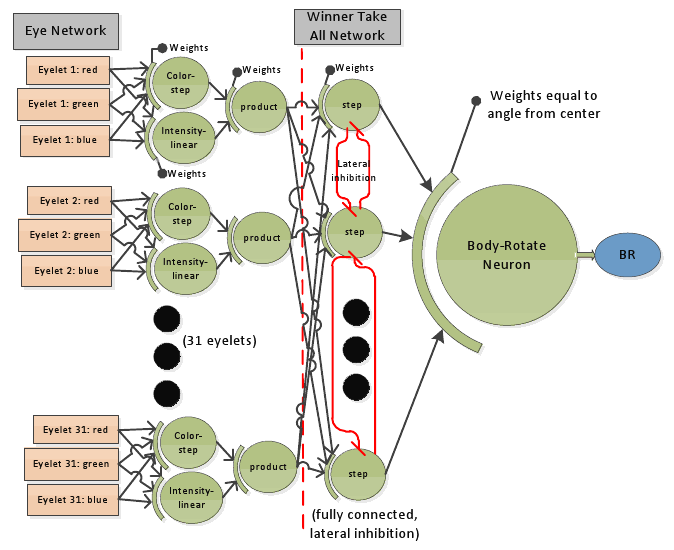
\includegraphics[scale=.5]{img/brain4.png}
  \caption{Brain 4's WTA eyelet network}
  \label{fig:brain4}
\end{center}
\end{figure}
